\documentclass[pra, onecolumn, notitlepage, floats, 11pt]{revtex4-1}

\usepackage[T1]{fontenc}
\usepackage{graphicx}
\usepackage{color}
\usepackage{latexsym,amsmath}
\usepackage{comment}
\usepackage{tabularx}
\usepackage{siunitx}
\usepackage{multirow}
\usepackage{mathtools}
\usepackage{tikz, fp}
\usepackage{wrapfig}
\usepackage{amsfonts}
\usepackage{bbold}
\usepackage[pdftex,colorlinks=true, pdfstartview=FitV, linkcolor=linkcolor, citecolor=linkcolor, urlcolor=linkcolor, hyperindex=true,hyperfigures=true]{hyperref} %hyperlink%
\usepackage{fancyhdr}
\usepackage{inconsolata}
\usepackage{listings}
\usepackage{physics}
\usepackage{datetime}
\usepackage[caption=false]{subfig}
\usepackage{titlesec}

\renewcommand{\figurename}{Figure}
\renewcommand{\tablename}{Table}
\renewcommand{\thetable}{\arabic{table}}

\definecolor{airforceblue}{rgb}{0.36, 0.54, 0.66}  %#5D8AA8
\definecolor{cobalt}{rgb}{0.0, 0.28, 0.67}         %#0047AB
\definecolor{coolblack}{rgb}{0.0, 0.18, 0.39}      %#002E63
\definecolor{dartmouthgreen}{rgb}{0.05, 0.5, 0.06} %#00693E
\definecolor{mydmg}{rgb}{0.05, 0.5, 0.06}          %#00693E
\definecolor{lava}{rgb}{0.81, 0.06, 0.13}          %#CF1020
\definecolor{myred}{rgb}{0.81, 0.06, 0.13}         %#CF1020
% move section headings to left
% \sffamily
% \scshape
%\titleformat{\section}{\raggedright\sffamily\bfseries\fontsize{13pt}{13}\selectfont}{\arabic{section}}{1em}{\MakeUppercase}
\titleformat{\section}{\raggedright\bfseries\scshape\fontsize{13pt}{13}\selectfont}{\color{cobalt}\arabic{section}}{1em}{\color{cobalt}}
\titleformat{\subsection}{\raggedright\bfseries\scshape\fontsize{12pt}{12}\selectfont}{{\color{cobalt}\arabic{section}.\arabic{subsection}}}{1em}{\color{cobalt}}
\renewcommand{\thesection}{\arabic{section}}
\renewcommand{\thesubsection}{\arabic{subsection}}
\renewcommand{\thesubsubsection}{\arabic{subsubsection}}
\makeatletter
\renewcommand{\p@subsection}{\thesection.}
\renewcommand{\p@subsubsection}{\thesection.\thesubsection.}
\makeatother


\linespread{0.956}

\DeclarePairedDelimiter\ceil{\lceil}{\rceil}
\DeclarePairedDelimiter\floor{\lfloor}{\rfloor}

\definecolor{linkcolor}{rgb}{0,0,0.65}
\definecolor{shadecolor}{rgb}{0.95, 0.95, 0.95}
\definecolor{mygreen}{rgb}{0,0.6,0}
\definecolor{mygray}{rgb}{0.5,0.5,0.5}
\definecolor{mymauve}{rgb}{0.58,0,0.82}
\lstdefinestyle{fortran}
{
    backgroundcolor=\color{shadecolor},       % background color
    basicstyle=\ttfamily\scriptsize,          % the size of the fonts that are used for the code
    breakatwhitespace=false,                  % sets if automatic breaks should only happen at whitespace
    breaklines=false,                         % sets automatic line breaking
    captionpos=b,                             % sets the caption-position to bottom
    commentstyle=\color{mygreen},             % comment style
    extendedchars=true,                       % lets you use non-ASCII characters; for 8-bits encodings only, does not work with UTF-8
    keepspaces=true,                          % keeps spaces in text, useful for keeping indentation of code (possibly needs columns=flexible)
    keywordstyle=\bfseries\color{blue},       % keyword style
    language=[95]Fortran,                     % the language of the code
    numbers=left,                             % where to put the line-numbers; possible values are (none, left, right)
    numbersep=5pt,                            % how far the line-numbers are from the code
    numberstyle=\tiny\color{mygray},          % the style that is used for the line-numbers
    rulecolor=\color{black},                  % if not set, the frame-color may be changed on line-breaks within not-black text (e.g. comments (green here))
    showspaces=false,                         % show spaces everywhere adding particular underscores; it overrides 'showstringspaces'
    showstringspaces=false,                   % underline spaces within strings only
    showtabs=false,                           % show tabs within strings adding particular underscores
    stepnumber=1,                             % the step between two line-numbers. If it's 1, each line will be numbered
    stringstyle=\color{mymauve},              % string literal style
    tabsize=4,                                % sets default tabsize to 4 spaces
    title=\lstname                            % show the filename of files
}

\lstdefinestyle{python}
{
    backgroundcolor=\color{shadecolor},       % background color
    basicstyle=\ttfamily\scriptsize,          % the size of the fonts that are used for the code
    breakatwhitespace=false,                  % sets if automatic breaks should only happen at whitespace
    breaklines=false,                         % sets automatic line breaking
    captionpos=b,                             % sets the caption-position to bottom
    commentstyle=\color{mygreen},             % comment style
    extendedchars=true,                       % lets you use non-ASCII characters; for 8-bits encodings only, does not work with UTF-8
    keepspaces=true,                          % keeps spaces in text, useful for keeping indentation of code (possibly needs columns=flexible)
    keywordstyle=\bfseries\color{blue},       % keyword style
    language=Python,                          % the language of the code
    numbers=left,                             % where to put the line-numbers; possible values are (none, left, right)
    numbersep=5pt,                            % how far the line-numbers are from the code
    numberstyle=\tiny\color{mygray},          % the style that is used for the line-numbers
    rulecolor=\color{black},                  % if not set, the frame-color may be changed on line-breaks within not-black text (e.g. comments (green here))
    showspaces=false,                         % show spaces everywhere adding particular underscores; it overrides 'showstringspaces'
    showstringspaces=false,                   % underline spaces within strings only
    showtabs=false,                           % show tabs within strings adding particular underscores
    stepnumber=1,                             % the step between two line-numbers. If it's 1, each line will be numbered
    stringstyle=\color{mymauve},              % string literal style
    tabsize=4,                                % sets default tabsize to 4 spaces
    title=\lstname                            % show the filename of files
}

\lstdefinestyle{bash}
{
    backgroundcolor=\color{shadecolor},       % background color
    basicstyle=\ttfamily\scriptsize,          % the size of the fonts that are used for the code
    breakatwhitespace=false,                  % sets if automatic breaks should only happen at whitespace
    breaklines=false,                         % sets automatic line breaking
    captionpos=b,                             % sets the caption-position to bottom
    commentstyle=\color{mygreen},             % comment style
    extendedchars=true,                       % lets you use non-ASCII characters; for 8-bits encodings only, does not work with UTF-8
    keepspaces=true,                          % keeps spaces in text, useful for keeping indentation of code (possibly needs columns=flexible)
    keywordstyle=\bfseries\color{blue},       % keyword style
    language=bash,                            % the language of the code
    numbers=left,                             % where to put the line-numbers; possible values are (none, left, right)
    numbersep=5pt,                            % how far the line-numbers are from the code
    numberstyle=\tiny\color{mygray},          % the style that is used for the line-numbers
    rulecolor=\color{black},                  % if not set, the frame-color may be changed on line-breaks within not-black text (e.g. comments (green here))
    showspaces=false,                         % show spaces everywhere adding particular underscores; it overrides 'showstringspaces'
    showstringspaces=false,                   % underline spaces within strings only
    showtabs=false,                           % show tabs within strings adding particular underscores
    stepnumber=1,                             % the step between two line-numbers. If it's 1, each line will be numbered
    stringstyle=\color{mymauve},              % string literal style
    tabsize=4,                                % sets default tabsize to 4 spaces
    title=\lstname                            % show the filename of files
}

\makeatletter
\newcommand{\srcsize}{\@setfontsize{\srcsize}{5pt}{5pt}}
\makeatother


\pagestyle{fancy}
\fancyhf{}
\fancyhead[L]{Rocco Ardino (Mat. 1231629)}
\fancyhead[R]{\bf\thepage}
\fancyfoot[L]{\textsc{report}: Week 9}
\fancyfoot[R]{\today}
\renewcommand{\headrulewidth}{0.1pt}
\renewcommand{\footrulewidth}{0.1pt}

\newcommand{\codebold}[2][cobalt]{\texttt{\bfseries {\color{#1}#2}}}
\newcommand{\code}[2][black]{\color{#1}\texttt{#2}}
\newcommand{\codefunctionbold}[2]{\texttt{\bfseries {\color{cobalt}#1}({\color{lava}#2})}}
\newcommand{\codefunction}[2]{\texttt{#1(#2})}










\begin{document}

\title{Quantum Information and Computing 2020/21\\Week 9 report}

\author{Rocco Ardino}

\date{\today}





\begin{abstract}
    In this work we deal with the monodimensional Ising model Hamiltonian. The first problem faced is to write the code needed for the initialization of the Hamiltonian for \( N \) spins, so for its \( 2^{N} \times 2^{N} \) matrix representation. Then, we exploit the Lapack library for the diagonalization and to find the eigenvalues. Lastly, the first energy levels are computed for several values of \( N \) and plotted with respect to the interaction strength in order to study the system.
\end{abstract}

\maketitle





\section{Theory}
The monodimensional Ising model describes a linear chain of \( N \) spins under the action of a magnetic field. The Hamiltonian describing such a system reads:
\begin{equation}
    \hat{H}
    =
    \lambda \sum_{i=1}^{N} \sigma_{i}^{z} + \sum_{i=1}^{N-1} \sigma_{i}^{x} \sigma_{i+1}^{x}
    \quad ,
    \label{eq:09_T_1}
\end{equation}
where \( \lambda \) is the interaction strength and the \( \sigma \)'s are the Pauli matrices, for which the following notation is employed:
\begin{align}
    \sigma_{i}^{z}
    &=
        \mathbb{1}_{1} \otimes \cdots \mathbb{1}_{i-1} \otimes \sigma_{i}^{z} \otimes \mathbb{1}_{i+1} \otimes \cdots \mathbb{1}_{N}    \\
    \sigma_{i}^{x} \sigma_{i+1}^{x}
    &=
        \mathbb{1}_{1} \otimes \cdots \mathbb{1}_{i-1} \otimes \sigma_{i}^{x} \otimes \sigma_{i+1}^{x} \otimes \mathbb{1}_{i+2} \otimes \cdots \mathbb{1}_{N}
        \quad .
\end{align}

In order to find the energy levels of the system, we should diagonalize the Ising Hamiltonian \( \hat{H} \). Then, by studying the eigenvalues, we expect for \( \lambda = 0 \) that the ground state is 2-fold degenerate and the first excited state is \( 2(N-1) \)-fold degenerate. The physical reason is due to the fact that with no field the only term remaining is the interaction one, so spins align along the \( x \)-axis. If we increase the value of \( \lambda \), we expect that the degeneracy disappears after a certain value of \( \lambda = \lambda_{c} \), over which a phase transition happens. However, in practice we can only deal with a small number of spins \( N \), so the degeneracy for \( 0 < \lambda < \lambda_{c} \) will be only ``approximate'' and it becomes more precise by increasing the number of spins \( N \).





\section{Code Development}
For this work, the new module \codebold{ising\_utils} is implemented, containing several functions and subroutines for multiple purposes:
\vspace{-5pt}
\begin{itemize}%[nolistsep]
    \setlength\itemsep{-3pt}
    \item \codefunctionbold{ising\_tensor\_prod}{mat1,mat2}, for executing the tensor product of the two input matrices \code{mat1} and \code{mat2};
    \item \codefunctionbold{ising\_identity}{N}, for instantiating the identity matrix for \code{N} spins, so of dimensions \( 2^{\code{N}} \times 2^{\code{N}} \);
    \item \codefunctionbold{ising\_hmat\_init}{N,L}, for initializing the Ising Hamiltonian for \code{N} spins and an interaction strength parameter \code{L};
    \item \codefunctionbold{ising\_hmat\_diag}{hmat,eigs}, for diagonalizing the Ising Hamiltonian and returning both the eigenfunctions (in the \code{hmat} input variable) and the eigenvalues (in \code{eigs});
    \item \codefunctionbold{ising\_print\_hmat\_std}{hmat,formatted}, for printing the Ising Hamiltonian matrix entries on standard output and in a formatted way, if specified.
\end{itemize}

Moreover, another module, namely \codebold{cmdline}, is implemented to have a command-line argument parser and for default arguments handling. In particular, we explain the new core functionalities of both the modules in the following subsections.



\subsection{Tensor product implementation}
The code to perform the tensor product operation between two input matrices is showed in Listing \ref{lst:08_C_SS_1_1}. This part is crucial for the Ising Hamiltonian initialization, since this task relies on the tensor product between \( 2 \times 2 \) identity and Pauli matrices.

\begin{lstlisting}[
    style=fortran,
    frame=single,
    label={lst:08_C_SS_1_1},
    caption={Implementation of the tensor product operation between two matrices.}
]
function ising_tensor_prod(mat1, mat2) result(res)
    complex(8), dimension(:,:) :: mat1                ! input  arguments
    complex(8), dimension(:,:) :: mat2                ! input  arguments
    complex(8), dimension(:,:), allocatable :: res    ! output result

    integer(4) :: N1, N2, M1, M2
    integer(4) :: ii, jj, lli, llj, uui, uuj

    N1 = size(mat1,1)
    N2 = size(mat2,1)
    M1 = size(mat1,2)
    M2 = size(mat2,2)

    allocate(res(N1*N2,M1*M2))

    ! loop to execute tensor product between mat1 and mat2
    do ii=1,N1
        do jj=1,M1
            lli = (ii-1)*N2 + 1
            llj = (jj-1)*M2 + 1
            uui =  ii   *N2
            uuj =  jj   *M2
            res(lli:uui,llj:uuj) = mat1(ii,jj)*mat2
        end do
    end do
end function ising_tensor_prod
\end{lstlisting}



\subsection{Ising Hamiltonian initialization}
The code to perform the initialization of the Ising Hamiltonian is showed in Listing \ref{lst:08_C_SS_2_1}. Given the number of spins in the linear chain and the interaction strength \( \lambda \), this function returns the \( 2^{N} \times 2^{N} \) Hamiltonian matrix needed for the following studies. Note how the crucial operation, which constitutes the bottleneck, is the tensor product part.

\begin{lstlisting}[
    style=fortran,
    frame=single,
    label={lst:08_C_SS_2_1},
    caption={Implementation of the Ising Hamiltonian initialization.}
]
function ising_hmat_init(N, L) result(hmat)
    integer(4) :: N                             ! input  arguments
    real(8)    :: L                             ! input  arguments
    complex(8), dimension(2**N,2**N) :: hmat    ! output result

    complex(8), dimension(2,2) :: s_x, s_z      ! Pauli matrices sx, sz
    integer(4) :: ii

    s_x      = COMPLEX( 0.0d0, 0.0d0)
    s_x(1,2) = COMPLEX( 1.0d0, 0.0d0)
    s_x(2,1) = COMPLEX( 1.0d0, 0.0d0)
    s_z      = COMPLEX( 0.0d0, 0.0d0)
    s_z(1,1) = COMPLEX( 1.0d0, 0.0d0)
    s_z(2,2) = COMPLEX(-1.0d0, 0.0d0)

    ! initialize Hamiltonian to zero
    hmat = COMPLEX(0.0d0, 0.0d0)
    ! fill with the first piece of Ising Hamiltonian
    do ii=1,N
        hmat = hmat + ising_tensor_prod(                  &
            ising_tensor_prod(ising_identity(ii-1), s_z), &
            ising_identity(N-ii)                          &
        )
    end do
    ! multiply by lambda the first piece
    hmat = COMPLEX(L,0.0d0) * hmat
    ! fill with the second piece of Ising Hamiltonian
    do ii=1,N-1
        hmat = hmat + ising_tensor_prod(   &
            ising_tensor_prod(                                &
                ising_tensor_prod(ising_identity(ii-1), s_x), &
                s_x                                           &
            ),                                                &
            ising_identity(N-ii-1)                            &
        )
    end do
end function
\end{lstlisting}



\subsection{Ising Hamiltonian diagonalization}
For the calculation of the eigenvalues and eigenvectors of the discretized Hamiltonian, the Lapack function \codebold[black]{zheev} is employed since the matrix we are working with is hermitian. Therefore, the subroutine \codebold[black]{ising\_hmat\_diag} is built as a wrapper of the Lapack function, as it is showed in Listing \ref{lst:09_C_SS_3_1}. Note that the input arguments are changed after the execution of this subroutine, storing then the \( j^{\text{th}} \) eigenfunction in the \( j^{\text{th}} \) column of \code{hmat} and all the eigenvalues in \code{eigs}.

\begin{lstlisting}[
    style=fortran,
    frame=single,
    label={lst:09_C_SS_3_1},
    caption={Implementation of the wrapper of \code{zheev} for Ising Hamiltonian diagonalization.}
]
subroutine ising_hmat_diag(hmat, eigs)
    complex(8), dimension(:,:) :: hmat    ! input arguments
    real(8),    dimension(:)   :: eigs    ! input arguments

    complex(8), dimension(:), allocatable :: work(:)
    complex(8), dimension(:), allocatable :: rwork(:)
    integer(4) :: lwork, info
    integer(4) :: N

    N     = size(hmat, 1)
    lwork = max(1,2*N-1)

    allocate(work(lwork))
    allocate(rwork(max(1, 2*N)))
    call zheev('V', 'U', N, hmat, N, eigs, work, lwork, rwork, info)
    deallocate(work)
    deallocate(rwork)
end subroutine ising_hmat_diag
\end{lstlisting}



\subsection{Main program}
Lastly, all the functions described before are employed in a main program, in which a command-line argument parser is implemented in order to obtain an easier handling of the parameters of the simulation. Moreover, this functionality is also capable of giving default values to the arguments when they are not given.
To make the program more user-friendly, a \code{-h} help option has been added and in the beginning of the execution all the arguments given are printed along with a flag: \codebold[red]{F} if a value is given for it, \codebold[dartmouthgreen]{T} if default is taken. An example of this functionality and of the way to start the program is showed in Listing \ref{lst:09_C_SS_4_1}. A complete list of the options is given in Table \ref{tab:09_C_SS_4_1}.

\begin{table}[!h]
\begin{minipage}[t]{0.48\textwidth}
    \raisebox{-\height}{
    {\footnotesize
    \begin{tabular}{cccc}
        \toprule
        Arg option    &   Arg name        &   Arg meaning   &   Default     \\
        \colrule
        \code{-N}    &   \code{nspins}  &   \( N \)                         &   \( 2 \) \\
        \code{-L}    &   \code{lambda}  &   \( \lambda \)                   &   \( 1 \) \\
        \code{-K}    &   \code{levels}  &   First \( k \) levels to print   &   \( 1 \) \\
        \code{-h}    &   \code{help}        &   print help          &           \\
        \botrule
    \end{tabular}
    }}
    \caption{Command-line arguments of the program.}
    \label{tab:09_C_SS_4_1}
\end{minipage}
\hfill
\begin{minipage}[t]{0.48\textwidth}
\begin{lstlisting}[
    style=bash,
    frame=single,
    escapechar=!,
    label={lst:09_C_SS_4_1},
    caption={Example of launch and user interface.}
]
!{\bfseries\color{dartmouthgreen}\$}! !{\bfseries\color{cobalt}./09.o}! !{\bfseries\color{lava}-N}! 10 !{\bfseries\color{lava}-K}! 4

Running with the following cmdline options:

N =	      10	default [T/F]: !{\bfseries\color{red}F}!
L =	     1.0	default [T/F]: !{\bfseries\color{dartmouthgreen}T}!
K =	       4	default [T/F]: !{\bfseries\color{red}F}!

-12.381489999654752
-12.082569625309047
-11.491406263829482
-11.192485889483818
\end{lstlisting}
\end{minipage}
\end{table}

After the parser, if no exception is found, a subroutine with the main execution is run, which in order:
\begin{itemize}
    \setlength\itemsep{-3pt}
    \item initializes the Ising Hamiltonian \( \hat{H} \) for \( N \) spins and for an interaction strength \( \lambda \);
    \item diagonalizes \( \hat{H} \) and computes the eigenvectors and, in particular, the eigenvalues;
    \item prints the first \( k \) eigenvalues of \( \hat{H} \).
\end{itemize}
Last but not least, the program must be compiled with the flag \code{-ffree-line-length-0}.

In order to automatize every step for different parameters for \( N \), \( \lambda \) and \( k \), a Python script is employed to run multiple batch executions for different sets of input parameters. The results for a fixed number of spins \( N \) and for variable \( \lambda \) are stored in appropriately labelled files.





\section{Results}
The main program is run requiring to print the first \( k = 4 \) eigenvalues of the Ising Hamiltonian. In particular, the cases analyzed are the ones for \( N = 4, 6, 8, 10 \) spins and for \( \lambda \in [0,3] \). The results for the ladders, plotted through a Gnuplot script, are showed respectively in Figures \ref{fig:09_R_1}, \ref{fig:09_R_2}, \ref{fig:09_R_3} and \ref{fig:09_R_4}. We can observe the following behaviour:
\begin{itemize}
    \setlength\itemsep{-3pt}
    \item \( \lambda = 0 \)\\
        This is the non-interacting case. There is a 2-fold degeneracy of the first energy level.
    \item \( \lambda > 0 \)\\
        This is the interacting case. The previously described 2-fold degeneracy of the non-interacting case is now broken, being however ``approximately'' true until a certain value of \( \lambda \) that depends on the number of spins.
\end{itemize}
So, we can observe how the value of \( \lambda_{c} \) where a phase transition occurs becomes higher when increasing \( N \). We expect it to converge for large values of \( N \).

Another study has been performed by plotting the ground state eigenvalue depending on the field strength \( \lambda \) and on the number of spins \( N \), after normalizing it for \( N - 1 \). This choice is due to the fact that the spins at the boundaries have only one neighbour and so, when considering their interaction, they weigh \( \frac{1}{2} \) each and not \( 1 \). The result can be seen in Figure \ref{fig:09_R_5}.

\begin{figure*}[!h]
    \centering
    \subfloat[][{\small \( N = 4 \)}]{
        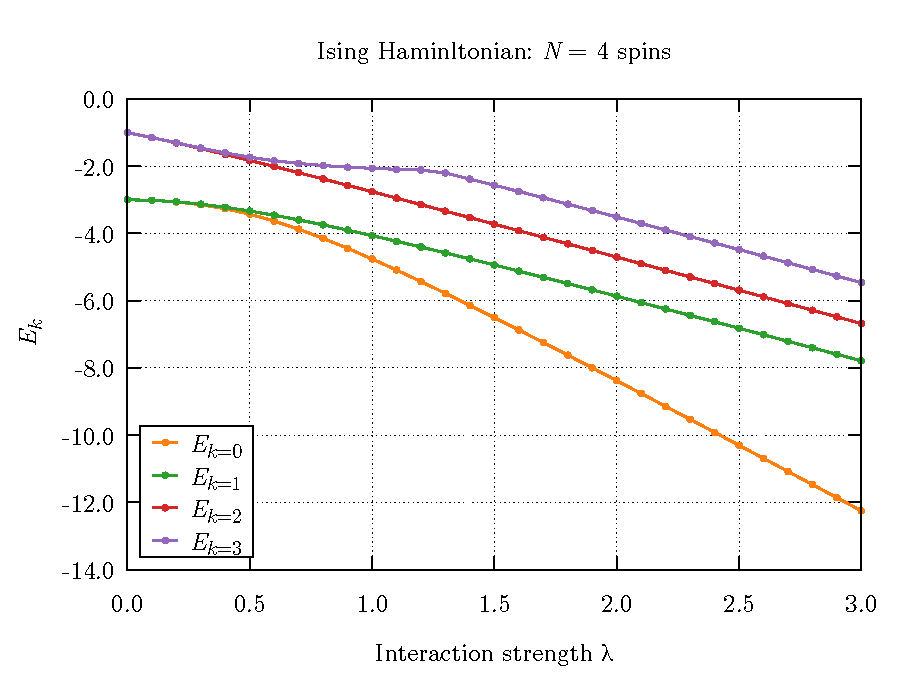
\includegraphics[width=0.48\textwidth]{images/ising_4_N.pdf}
        \label{fig:09_R_1}
    }
    \hfill
    \subfloat[][{\small \( N = 6 \)}]{
        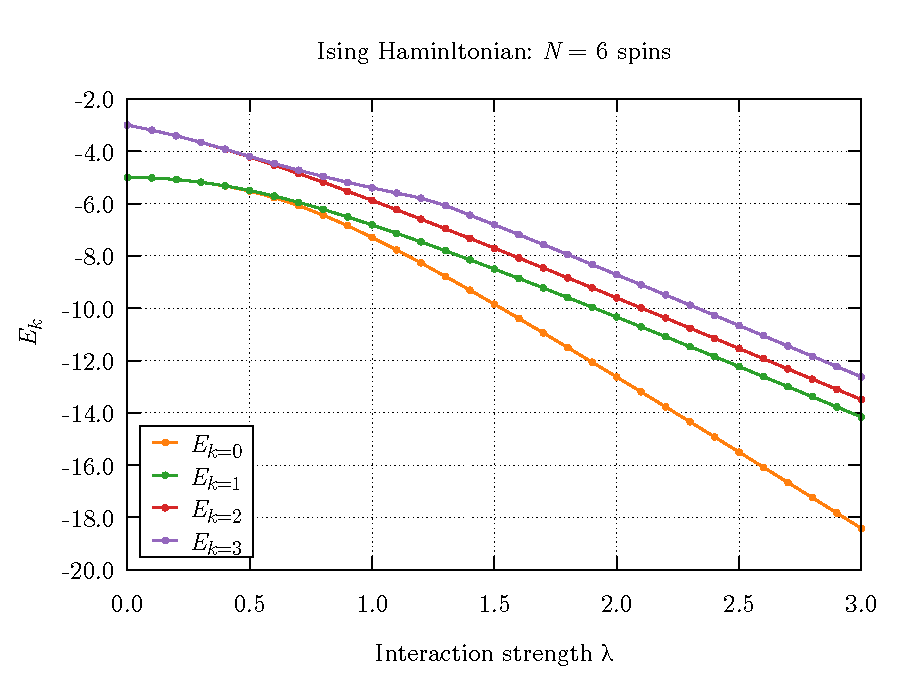
\includegraphics[width=0.48\textwidth]{images/ising_6_N.pdf}
        \label{fig:09_R_2}
    }

    \subfloat[][{\small \( N = 8 \)}]{
        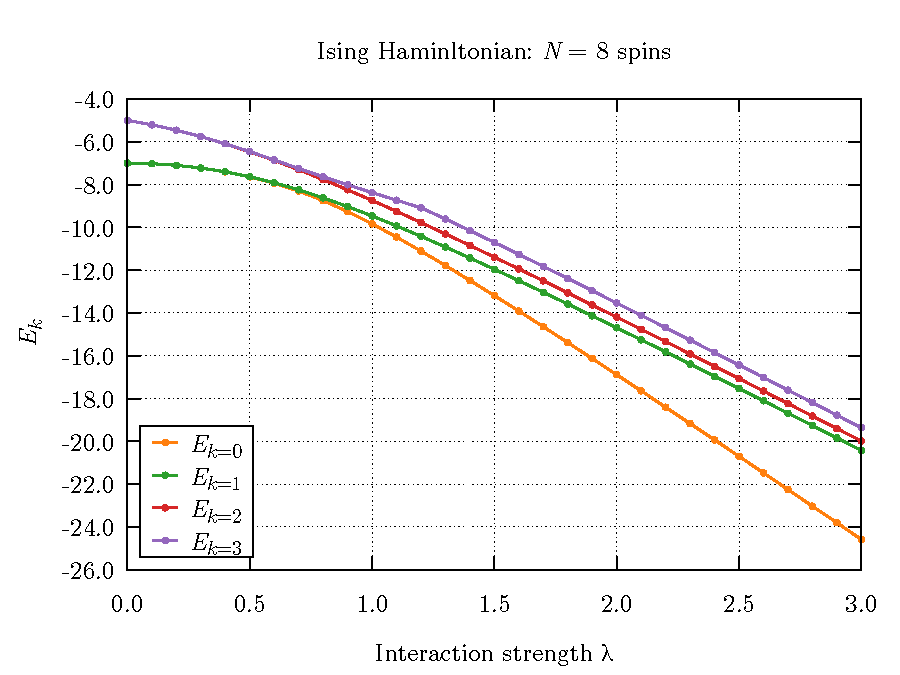
\includegraphics[width=0.48\textwidth]{images/ising_8_N.pdf}
        \label{fig:09_R_3}
    }
    \hfill
    \subfloat[][{\small \( N = 10 \)}]{
        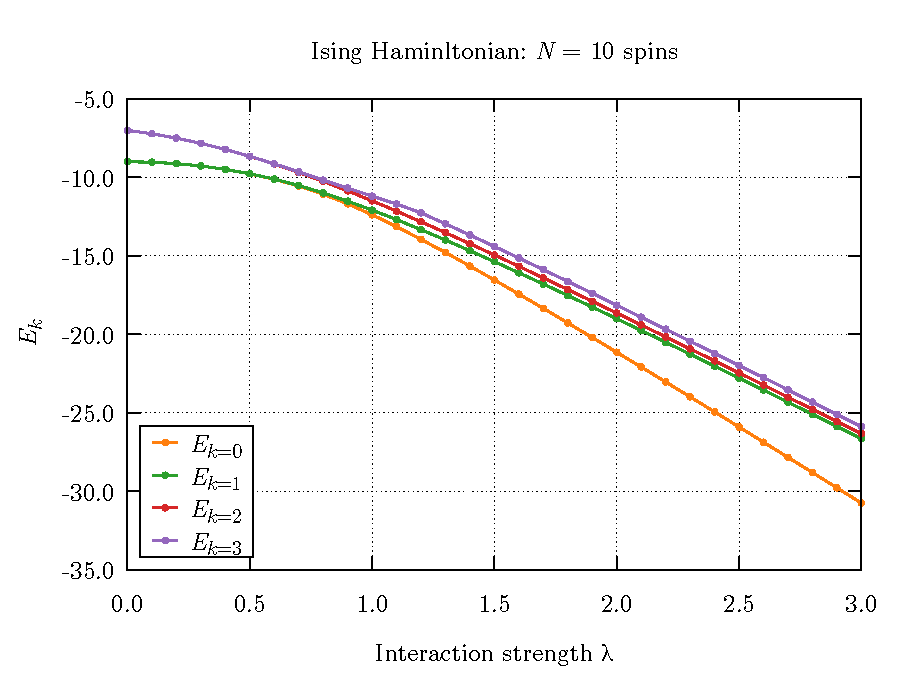
\includegraphics[width=0.48\textwidth]{images/ising_10_N.pdf}
        \label{fig:09_R_4}
    }
    \caption{First \( k = 4 \) eigenvalues of Ising Hamiltonian depending on the interaction strength \( \lambda \), for several number of spins \( N \).}
    \label{fig:09_R_1234}
\end{figure*}

\begin{figure*}[!h]
    \centering
    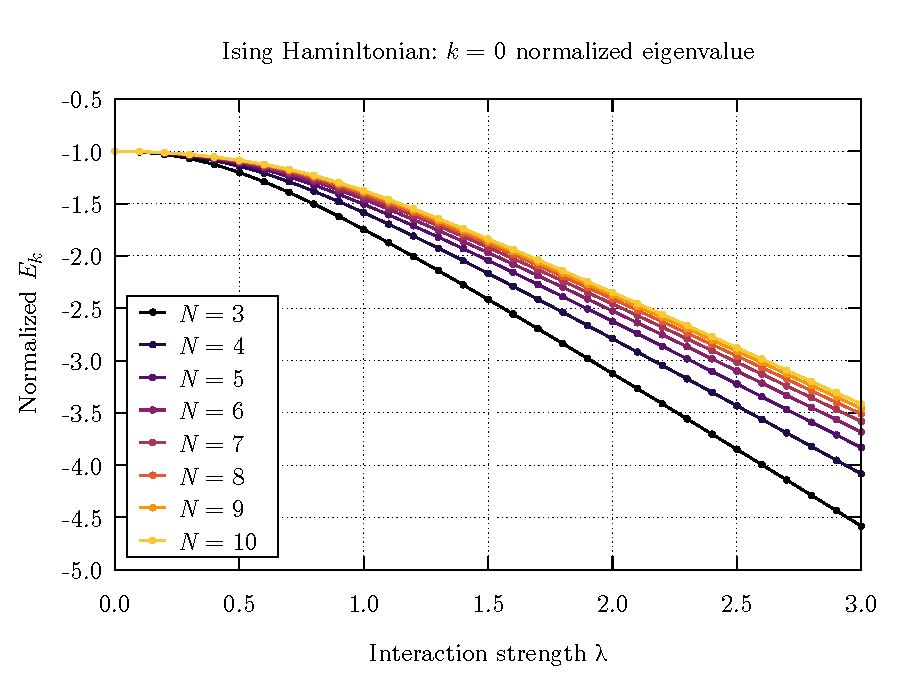
\includegraphics[width=0.48\textwidth]{images/ising_0_K.pdf}
    \caption{First \( k = 0 \) eigenvalue of Ising Hamiltonian depending on the interaction strength \( \lambda \) and for several number of spins \( N \), normalized by \( N - 1 \).}
    \label{fig:09_R_5}
\end{figure*}





\section{Self-evaluation}
In this work we have successfully tackled the problem of Ising model simulation with a certain number of spins \( N \) and with an input interaction strength \( \lambda \). The simulations showed in the results have been run for a maximum \( N = 10 \). However the machine on which the code is run is capable of reaching an \( N_{\mathrm{max}} = 14 \). In order to perform systematic studies for variable \( \lambda \) and for \( N > 10 \) a different and more efficient implementation should be written, in particular for the Hamiltonian initialization. The code written performs all the tensor products needed for this operation. This is the most complete and generic way to solve the task, however, it significantly slows the execution for large values of \( N \). An hard-coded and efficient solution could be employed, but the most complete one has been chosen for a better understanding.

\end{document}
